\documentclass[Thesis.tex]{subfiles}
\begin{document}

\chapter{Robot localization and Bayes filters}

\section{Robot localization}

Robot localization is the process of determining a robot's pose in a known environment. A common application for it is to find the starting position for planning algorithms. Thrun et al. distinguish between three different kinds of localization problems: \emph{Local localization}, \emph{global localization}, and the \emph{kidnapped robot problem}\cite{ThrunBurgardFox:2005}. The local localization problem keeps track of the robot's pose from a known initial pose and is considered the easiest problem of the three, since the error rate in position tracking is small and efficient algorithms exist to reduce it even further, like the Kalman filter and its derivatives\cite{ThrunBurgardFox:2005}. The global localization problem deals with finding the pose in a map without knowing the initial pose. It is an extension to the local localization problem and more difficult. But once the robot has found its pose, the problem degenerates into a local localization problem. However, when the robot is relocated by someone, it loses track of its pose. This is the kidnapped robot problem, which is the most difficult of the three localization problems.

All three problems have in common that they need a suitable environment representation, a map of the robot's whereabouts. There is a similar class of problems which are referred to as \gls{SLAM} problems. In these scenarios there is no prior map given, which makes the problems even more difficult. 

%The algorithm presented in this thesis will deal with the global localization problem and will also be able to recover from a kidnapped robot situation.

\section{Bayes filters}
A good way to model localization problems are Bayes filters. They make use of Bayes' theorem to calculate the probability of a pose $x$ at time $t$ by accounting for the probability at time $t-1$ and the likelihood of the current pose. The Bayes' theorem is as follows:
%
\begin{align}
\p[P]{X}{Y} = \frac{ \p[P]{Y}{X} P(X) } { P(Y) }
\end{align}

In this equation, $P$ denotes the \gls{pdf} of a random variable. $\nicefrac{1}{P(Y)}$, commonly called $\eta$, is the normalization factor. It is usually derived by marginalization: 
\begin{align}
P(Y) = \sum\limits_i \p[P]{Y}{x_i}
\end{align}
In a continuous approach the sum is replaced by an integral, but for the algorithm in this thesis the discrete version is sufficient. $P(X)$ is the prior, a previous assumption.
%, defaulting to a uniformly \gls{iid} random variable. 
The likelihood, the last factor needed for the calculations, can be found in $\p[P]{Y}{X}$. One can read it as the \emph{probability of $Y$ given $X$}, that means the probability of event $Y$ when event $X$ was observed. 
The likelihood is a very important part of the algorithm and will be described in detail in \algRef{alg:eval}. All together Bayes' theorem is used to calculate the posterior probability of $X$ given $Y$. That is the probability that event $X$ happens when event $Y$ is observed. In other words this means that the current probability for $X$ given $Y$ is derived by calculating how likely event $Y$ is, given event $X$ regarding $X$'s sole probability. 

It should be noted that throughout the rest of this thesis prior and posterior probabilities will be called prior and posterior beliefs, respectively. This terminology has a simple reason: Although a robot does not have beliefs as we use the word in terms of human thoughts, it fits the context better. Probability might imply that the algorithm would try to \emph{predict} the robot's future position---belief on the other hand describes a theoretical possible \emph{current} state.

\bigskip

By using Bayes' theorem over several time steps, it is possible to implement a Markov chain model. A Markov chain model describes a system in which the Markov assumption holds, which says that the state of a system at time $t$ can be calculated by just knowing the state at time $t-1$ but no other states, thus being independent from the others.

\begin{algorithm}
\caption{Bayes filter}
\label{alg:bayesfilter}
\SetKwProg{bayesfilter}{bayes\mathunderscore f{i}lter}{}{end}
\SetKwData{truevalue}{true}
\SetKwData{guess}{best\mathunderscore guess}
\SetKwData{belief}{best\mathunderscore belief}

\bayesfilter{} {
  \belief = 0\;
  \guess = null\;
  \While{\truevalue}{
    \ForEach{$x_t$} {
      bel$(x_t) = \eta$ likelihood$(x_t)$ bel$(x_{t-1})$\;
      \If{bel$(x_t) > $\belief}{
        \belief = bel$(x_t)$\;
        \guess = $x_t$\;
      }
    }
  }
}
\end{algorithm}

This simple \algRef{alg:bayesfilter} is the basic form of a Bayes filter. Its purpose is to find a state estimation by \emph{updating} the beliefs (bel($x_t$)) for each state $x$ during every time step $t$ and eventually converging to a value close to the true value. This is done by using the former posterior beliefs as priors for the new posterior beliefs.
The state with the highest belief is the likeliest.

\subsection{The door example}
\begin{figure}
  \centering
  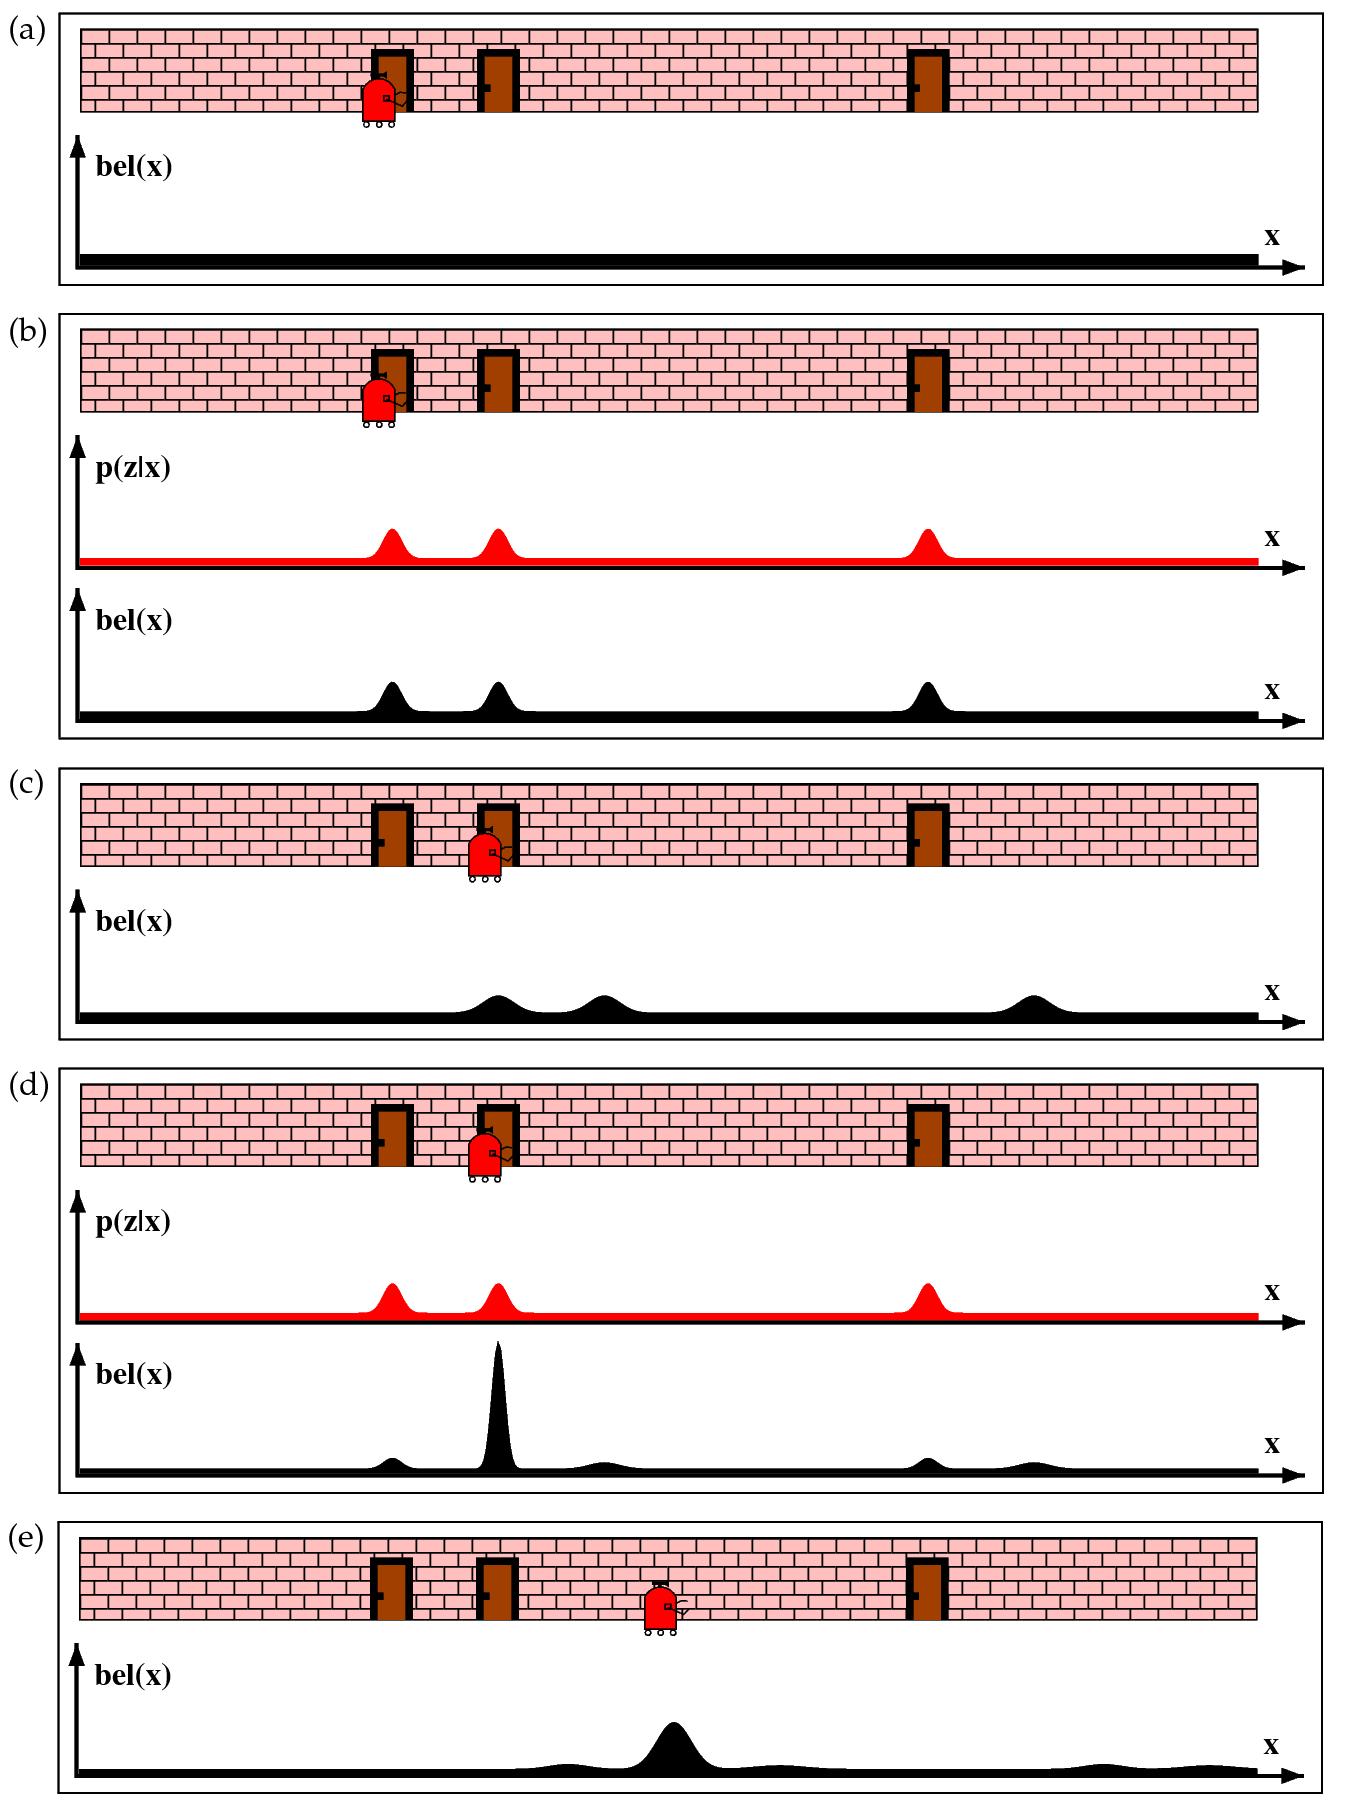
\includegraphics[width=.9\columnwidth]{markov_localization}
  \caption{Markov localization: A one dimensional corridor with indistinguishable doors. From \cite[p.~6]{ThrunBurgardFox:2005}.}
  \label{fig:markov_localization_one_dimension}
\end{figure}

A popular example for demonstrating Bayes filters is the door example, which is illustrated in \figRef{fig:markov_localization_one_dimension}. A robot which can only move in one dimension and only sense whether it is in front of one of many indistinguishable doors or not shall localize itself in a corridor. 

At the time of initialization the robot has no information, thus its believe to be at a specific position is uniformly distributed (see \figRef{fig:markov_localization_one_dimension}(a), $bel(x)$).

After the initialization the robot uses its sensor to search for a door. It finds out that in fact it is located in front of one, so it applies a high likelihood for all positions which are in front of doors (see \figRef{fig:markov_localization_one_dimension}(b), \p{x}{z} where $z$ corresponds to sensor measurement). Now the prior belief $bel(x)$ and the likelihood \p{z}{x} are used to calculate the posterior belief \p{x}{z}, which is again called $bel(x)$.
%
\begin{align}
\p{x}{z} &= \eta\: \p{z}{x} bel(x) \label{eq:door_bayes}
\end{align}

A repeated measurement would add little information to the robot's belief. So the best solution to get more information is to move around a little and check for doors again. This can be seen in \figRef{fig:markov_localization_one_dimension}(c). Especially noteworthy is that the $bel(x)$ distribution is flattened a little bit. This is done to account for inaccuracies in the movement of robots.

During the next time step \formRef{eq:door_bayes} will be used again, with the new normalized belief and a new measurement. Since the robot again senses a door the robot first assigns high likelihoods for the doors, it then calculates the posterior belief. This leads to a considerable high value for the position close to the second door, we say the pose estimation converges to the real value. 

During the next movement the $bel(x)$ distribution flattens again, until the robot senses a new door. With the new information about this landmark the robot will be able to update his beliefs accordingly.

\end{document}